\documentclass[12pt]{article}
\usepackage[top=1in,left=1in, right = 1in, footskip=1in]{geometry}

\usepackage{graphicx}
%\usepackage{adjustbox}

%% \newcommand{\comment}{\showcomment}
\newcommand{\comment}{\nocomment}

\newcommand{\showcomment}[3]{\textcolor{#1}{\textbf{[#2: }\textsl{#3}\textbf{]}}}
\newcommand{\nocomment}[3]{}

\newcommand{\jd}[1]{\comment{cyan}{JD}{#1}}
\newcommand{\swp}[1]{\comment{magenta}{SWP}{#1}}

\newcommand{\eref}[1]{(Eq.~\ref{eq:#1})}
\newcommand{\fref}[1]{Fig.~\ref{fig:#1}}
\newcommand{\Fref}[1]{Fig.~\ref{fig:#1}}
\newcommand{\sref}[1]{Sec.~\ref{#1}}
\newcommand{\frange}[2]{Fig.~\ref{fig:#1}--\ref{fig:#2}}
\newcommand{\tref}[1]{Table~\ref{tab:#1}}
\newcommand{\tlab}[1]{\label{tab:#1}}
\newcommand{\seminar}{SE\mbox{$^m$}I\mbox{$^n$}R}

\usepackage{amsthm}
\usepackage{amsmath}
\usepackage{amssymb}
\usepackage{amsfonts}

% \usepackage{lineno}
% \linenumbers

\usepackage[pdfencoding=auto, psdextra]{hyperref}

\usepackage{natbib}
\bibliographystyle{chicago}
\date{\today}

\usepackage{xspace}
\newcommand*{\ie}{i.e.\@\xspace}

\usepackage{color}

\newcommand{\Rx}[1]{\ensuremath{{\mathcal R}_{#1}}} 
\newcommand{\Ro}{\Rx{0}}
\newcommand{\RR}{\ensuremath{{\mathcal R}}}
\newcommand{\Rhat}{\ensuremath{{\hat\RR}}}
\newcommand{\tsub}[2]{#1_{{\textrm{\tiny #2}}}}

\begin{document}

\begin{flushleft}{
	\Large
	\textbf\newline{
		Estimating the effects of social distancing on preventing the spread of coronavirus disease 2019 (COVID-19) in South Korea
	}
}
\end{flushleft}

\pagebreak

Here, we use traffic data to compare and contrast the potential role of social distancing in preventing the spread of COVID-19 in two geographically separated major cities in South Korea.

\section{Data description}

Here, we analyze epidemiological data, collected bewteen January 20--March 16, 2020, describing the COVID-19 outbreak in Korea.
Daily number of reported cases in each geographic region was transcribed from press releases by Korea Centers for Disease Control and Prevention (KCDC).
Partial line lists were transcribed from press releases and reports from KCDC and various local and provincial government websites.
All data and original reports are stored in a publicly available GitHub repoository: https://github.com/parksw3/COVID19-Korea.

\begin{figure}[!h]
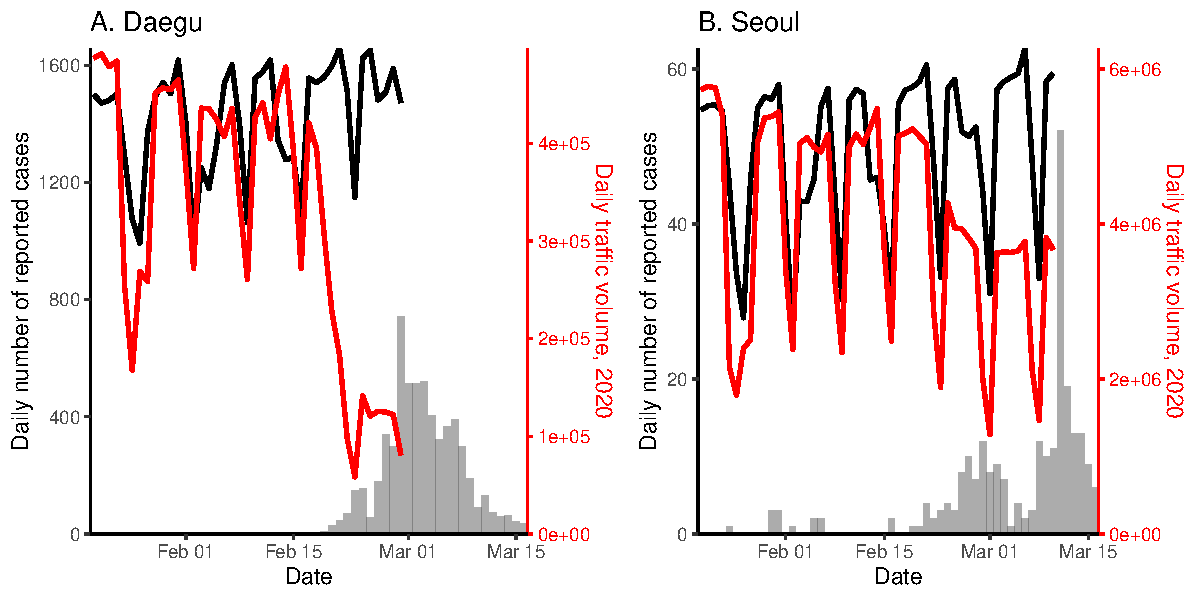
\includegraphics[width=\textwidth]{figure_compare_report.pdf}
\caption{
\textbf{Comparison of epidemiological and traffic data from Daegu and Seoul.}
Solid lines represent the daily metro traffic volume in 2020 (red) and in 2017--2019 (gray).
Black lines represent the average daily metro traffic volume in previous years.
}
\label{fig:data}
\end{figure}

We focus our analysis on two cities in which the biggest number of COVID-19 cases have been reported: Daegu and Seoul.
Bewteen January 20--March 16, 2020, 6,083 cases were reported from Daegu and 248 from Seoul.
Need one or two sentences about epidemic.

Daily metro traffic from Daegu and Seoul were obtained from their corresponding government websites.
Need one or two sentences about metro. 
About 80\% decrease in Daegu and 50\% decrease in Seoul after the identification of the church-related case.

%% https://www.data.go.kr/dataset/15002503/fileData.do
%% https://data.seoul.go.kr/dataList/OA-12914/S/1/datasetView.do

\section{Effective reproduction number}

We first estimate the time-varying effective reproduction number $R_t$ for both epidemics.
We account for changes in case definition by scaling the number of reported cases by the relative detection rate (i.e., a proportion of cases tested positive based a case definition divided by the mean detection rate among case definitions); 
using a narrow case definition is more likely to have a higher detection rate and a lower reporting rate than a wide one.
Likewise, we account for changes in the number of tests by scaling the number of reported cases again by the relative number of tests performed on each day; this step is performed separately for each case definition because the widening of a case definition necessarily increases the number of tests.

We then reconstruct the incidence time series from the scaled time series of reported cases by using the backward confirmation-to-onset delay distribution, inferred from the partial line list, and previously estimated incubation period distribution.
To account for right-censoring (i.e., cases that are infected but have not been reported yet), we estimate the forward onset-to-confirmation delay distribution and estimate the probability that a case infected on a given day will be reported before March 16, 2020. 
Then, we divide the reconstructed incidence time series by this probability and estimate the effective reproduction number using the renewal equation using a 14-day sliding window.
We only calculate the effective reproduction number until March 10, 2020 because the degree of right-censoring too large afterwards.

\begin{figure}[!ht]
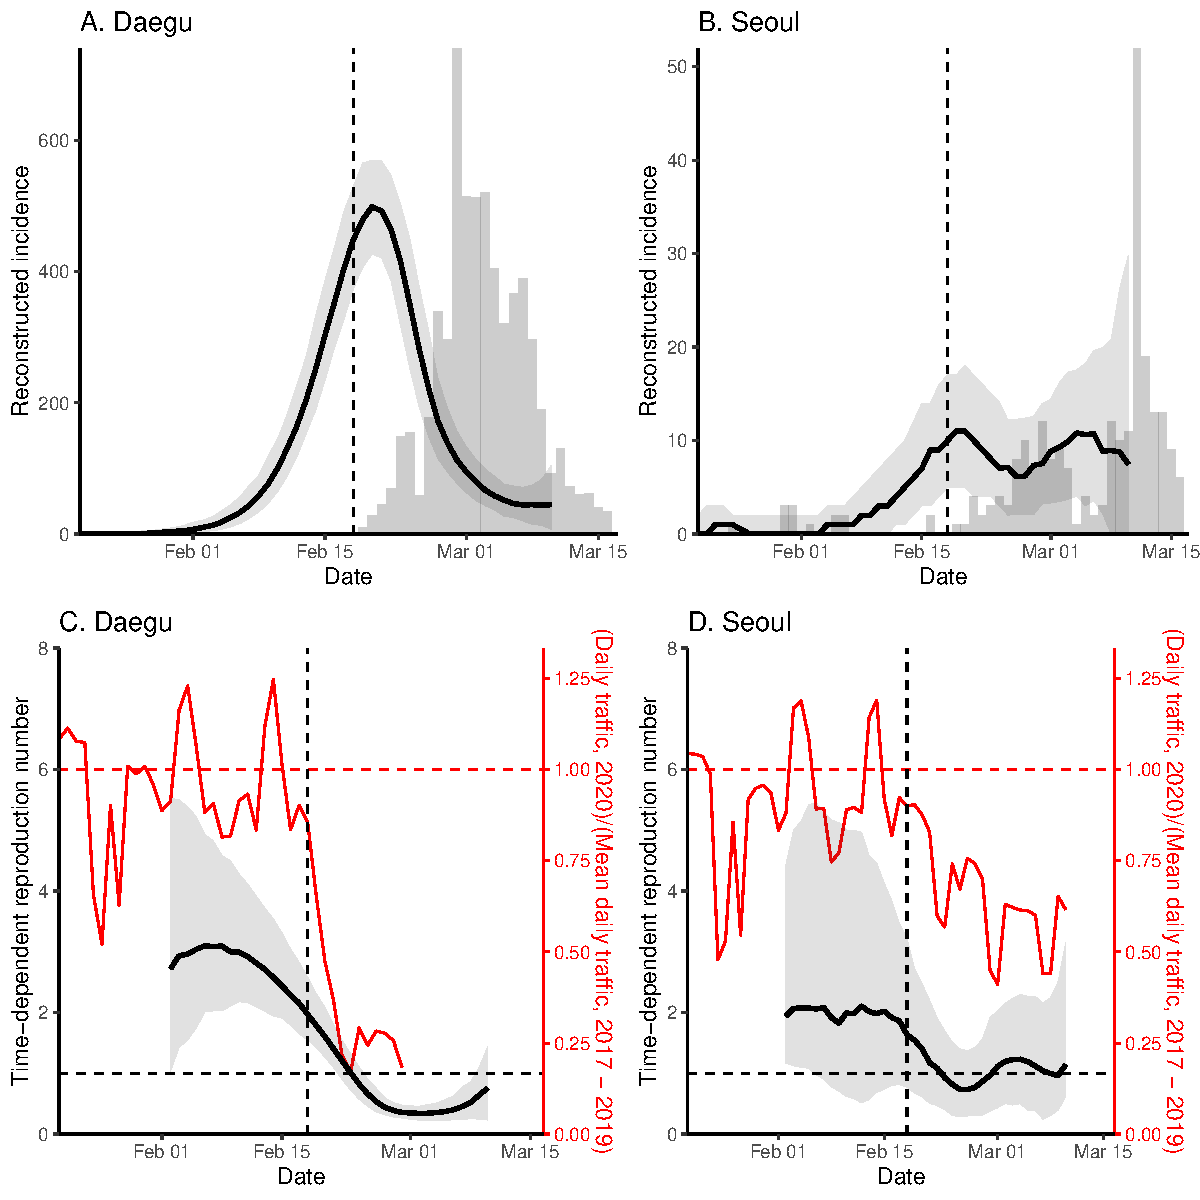
\includegraphics[width=\textwidth]{figure_compare_R_t.pdf}
\caption{
\textbf{Comparison of effective reproduction number and reconstructed incidence time series in Daegu and Seoul.}
}
\label{fig:eff}
\end{figure}

\fref{eff} compares the estimates of $R_t$ in Daegu and Seoul.
While $R_t$ drops below 1 in Daegu shortly after its first case was confirmed (February 18, 2020), 
the decrease is unclear in Seoul.
Similar patterns in $R_t$ can be found in adjacent provinces -- a sharp decrease in Gyeongsangbuk-do, which surrounds Daegu, and a persistent $R_t$ around 1 in Gyeonggi-do, which surrounds Seoul (Supplementary Materials).

\section{Effect of social distancing on the effective reproduction number}

\begin{figure}[!ht]
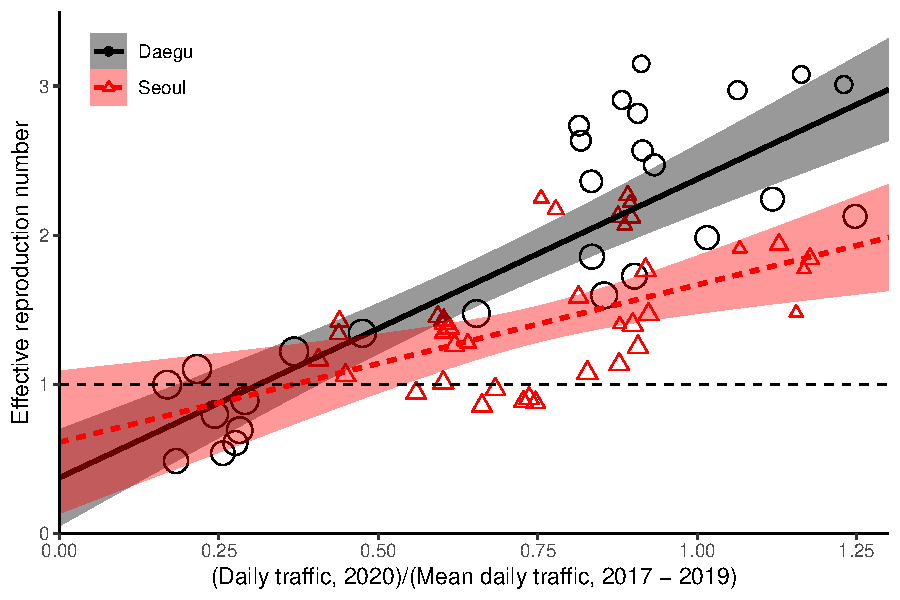
\includegraphics[width=\textwidth]{figure_traffic_regression.pdf}
\caption{
\textbf{Relationship between daily traffic volume and effective reproduction number.}
}
\label{fig:traffic}
\end{figure}

\begin{itemize}
  \item Traffic negatively correlated with $R_t$
  \item Geographically differential effect of traffic on $R_t$; other routes of transportation, other factors we don't consider
  \item Even if we can get traffic to 0 in Seoul, $R_t$ is not less than 1...?
\end{itemize}

\section{Discussion}

\begin{itemize}
  \item Provides indirect evidence of effect of social distancing on epidemic dynamics
  \item But social distancing alone might not be sufficient... others have said something
  \item SK might need stronger intervention in some places
\end{itemize}

Caveats:
\begin{itemize}
  \item Only two cities...although two coupled provinces show strikingly similar patterns
  \item Correlation not causation
  \item Did not account for geographic heterogeneity in testing or etc. Estimation of delay distribution etc all based on national line list.
\end{itemize}

\pagebreak

\section{Supplementary Materials}

\begin{figure}[!ht]
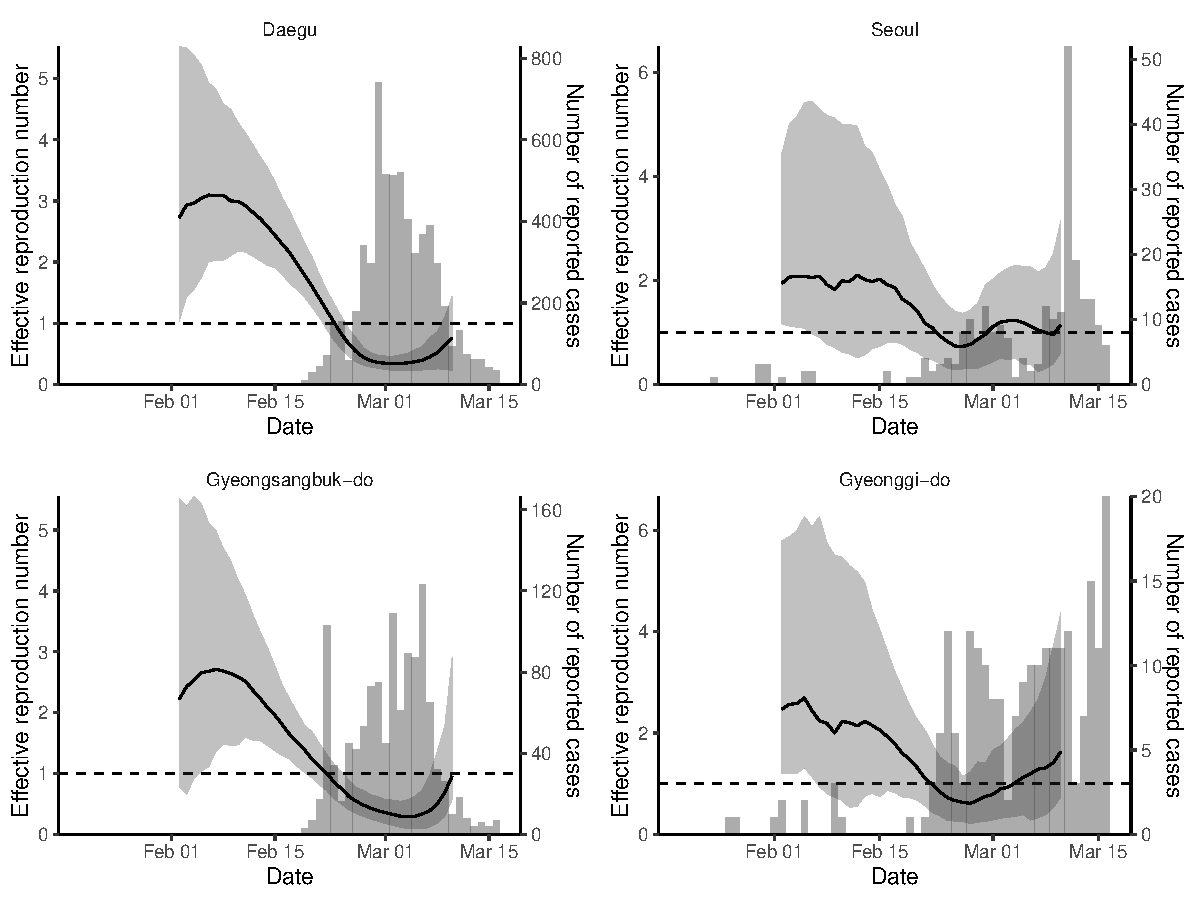
\includegraphics[width=\textwidth]{figure_R_t_all.pdf}
\caption{
\textbf{Comparison of effective reproduction number in Daegu, Seoul, Gyeongsangbuk-do, and Gyeonggi-do.}
}
\label{fig:eff}
\end{figure}

\end{document}
